\lecture{7}{14. April 2026}{Root Locus Method, II}

\section{PID Controllers}
A PID-controller (Proportional-Integral-Derivative) takes the error signal
\begin{equation*}
  e(t) = r(t) - y(t)
\end{equation*}
and turns it into a control input $u(t)$ for a plant/process.
A block diagram for how this process might look is shown on \Cref{fig:PID}.
\begin{figure} [ht]
  \centering
  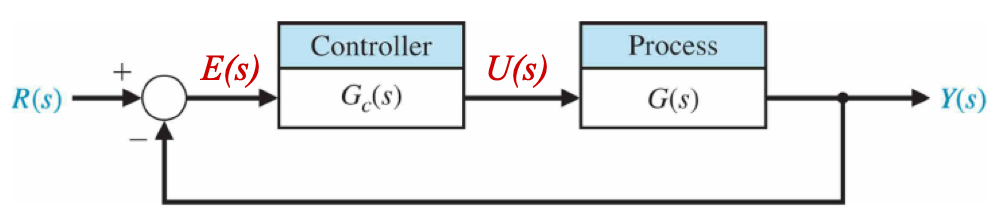
\includegraphics[width=0.8\linewidth]{./figures/PID.png}
  \caption{Block diagram of a simple process with a controller and feedback.}
  \label{fig:PID}
\end{figure}

The controller is
\begin{equation*}
  u(t) = K_P e(t) + K_I \int e(t) \, \mathrm{d}t + K_D \frac{\mathrm{d}e(t)}{\mathrm{d}t} 
\end{equation*}
or in the $s$-domain
\begin{equation} \label{eq:PIDs}
  G_c(s) = K_P + \frac{K_I}{s} + K_D s
.\end{equation}
Here, the three terms $K_P$, $K_I$, and $K_D$ each correspond to different elements as shown in \Cref{tab:PID}.
\begin{table}[ht]
  \centering
  \caption{Meaning of the different terms in a PID-controller.}
  \label{tab:PID}
  \begin{tabular}{|c|c|c|}
    \hline
    \textbf{Term}                            & \textbf{Meaning} & \textbf{Effect}                                  \\ \hline
    $K_P e(t)$                               & Proportional     & Reacts to present error                          \\ \hline
    $K_I \int e(t) \, \mathrm{d} t$          & Integral         & Reacts to past error; Removes steady-state error \\ \hline
    $K_D \frac{\mathrm{d}e(t)}{\mathrm{d}t}$ & Derivative       & Reacts to change in error; Adds damping          \\ \hline
  \end{tabular}
\end{table}
In this way, the output of a PID-controller is based on both the present error, the past accumulated error, and the rate in change of the error.

\subsection{Forms of PID Controllers}
The ideal derivative term in \Cref{eq:PIDs} is written as $K_D s$, however, a pure differentiator is usually not implemented directly, as it amplifies high frequency noise.
In practice, the derivative part is often filtered as
\begin{equation*}
  G_d(s) = \frac{K_D s}{\tau_{d} s + 1}
\end{equation*}
which is approximately equal to $K_D s$ when $\tau_d$ is very small compared with the process time constants.

It is also possible to leave out the derivative part entirely leaving you with a PI-controller with transfer function:
\begin{equation*}
  G_c(s) = K_P + \frac{K_I}{s}
.\end{equation*}
Or a PD-controller with transfer function:
\begin{equation*}
  G_c(s) = K_P + K_D s
.\end{equation*}
A PI-controller is common when steady-state error matters, whereas a PD-controller is more common when damping/overshoot reduction is important but the integral action is not as useful.

\subsubsection{PID as a Cascade of PI and PD}
A PID-controller can be interpreted as a PI controller followed by a PD controller:
\begin{equation*}
  G_c(s) = G_{PI}(s) G_{PD}(s)
\end{equation*}
where
\begin{align*}
  G_{PI}(s) &= \hat{K}_P + \frac{\hat{K}_I}{s} \\
  G_{PD}(s) &= \overline{K}_P + \overline{K}_D s
.\end{align*}
Multiplying these (as we do when combining cascading blocks) gives
\begin{equation*}
  G_C(s) = \left( \hat{K}_P + \frac{\hat{K}_I}{s} \right) \left( \overline{K}_P + \overline{K}_D s \right) = \hat{K}_P \overline{K}_P + \hat{K}_P \overline{K}_Ds + \frac{\hat{K}_I \overline{K}_P}{s} + \hat{K}_I \overline{K}_D
.\end{equation*}
We see that this is a PID-controller with
\begin{align*}
  K_P &= \overline{K}_P \hat{K}_P + \hat{K}_I \overline{K}_D \\
  K_D &= \hat{K}_P \overline{K}_D \\
  K_I &= \hat{K}_I \overline{K}_P
.\end{align*}

\subsubsection{Pole-zero interpretation of a PID controller} \label{sec:pzPID}
We use the general form of the transfer function for a PID controller, \Cref{eq:PIDs}, and put everything over a common denominator
\begin{equation*}
  G_c(s) = \frac{K_D s^2 + K_P s + K_I}{s}
.\end{equation*}
Factoring out $K_D$ we get:
\begin{equation*}
  G_C (s) = \frac{K_D \left( s^2 + \frac{K_P}{K_D}s + \frac{K_I}{K_D} \right)}{s}
.\end{equation*}
Then the quadratic part of the numerator can be written as
\begin{equation*}
  s^2 + \alpha s + b, \qquad  \alpha = \frac{K_P}{K_D}, \quad b = \frac{K_I}{K_D}
,\end{equation*}
which can be factored to $(s+z_1)(s+z_2)$.
So:
\begin{equation*}
  G_c(s) = \frac{K_D(s + z_1)(s+z_2)}{s}
.\end{equation*}
This means a PID-controller contributes one pole at $s = 0$ and two zeros determined by $K_P$, $K_I$, and $K_D$.
The pole at the origin comes from the integral term, $K_I / s$.
The two zeros come from the numerator:
\begin{equation*}
  K_D s^2 + K_p s + K_I
.\end{equation*}
By choosing $K_P$, $K_I$, and $K_D$, you change where these zeros are located.
In root locus design this is powerful as these zeros can then be used to pull the root locus toward the desired regions of the $s$-plane.

\subsection{PID Tuning}
As mentioned in \Cref{sec:pzPID}, the values of $K_P$. $K_I$, and $K_D$ can be tuned to change the root locus. 
This can generally be done in two different ways, namely via manual trial-and-error tuning with minimal analytic analysis using step responses and via Ziegler-Nichols tuning, which is a more analytic tuning method based on closed- and open-loop response to a step input.

\subsubsection{Manual PID Tuning}
Manual tuning starts by simplifying the controller as much as possible by setting $K_I = K_D = 0$, so initially we only have
\begin{equation*}
  G_c(s) = K_P
.\end{equation*}
Which means, first we must tune a proportional controller.
We then increase $K_P$ until the closed-loop system is just about unstable, before we reduce $K_P$ until the response has roughly quarter-amplitude decay.
Then we increase $K_I$ and $K_D$ manually to improve the step response.
Here, ``quarter-amplitude decay'' means that oscillations die out such that each overshoot peak os about one quarter of the previous overshoot peak.
This is a classic tuning target as it is neither too sluggish nor too oscillatory for most applications.

\paragraph{Effect of each PID gain}
\Cref{tab:PIDq} summarizes the usual qualitative effects of increasing each PID gain.
\begin{table}[ht]
  \caption{Qualitative effect of increasing each PID gain}
  \label{tab:PIDq}
\begin{tabular}{|c|c|c|l|}
\hline
\textbf{Increasing} & \textbf{Overshoot} & \textbf{Settling Time} & \textbf{Steady-state error} \\ \hline
$K_P$               & Increases          & Small/minimal effect   & Decreases                   \\ \hline
$K_I$               & Increases          & Increases              & Removes steady-state error  \\ \hline
$K_D$               & Decreases          & Decreases              & Little/no direct effect     \\ \hline
\end{tabular}
\end{table}
The intuition here is that $K_P$ pushes harder when the error is large.
This usually makes the system respond faster, but it can also lead to more overshoot.
$K_I$ keeps accumulating error over time, which is excellent for removing steady-state error, but it often makes the system more oscillatory.
$K_D$ reacts to the rate of change of the error acting like a damper.
It tends to reduce overshoot and make oscillations die out faster.

\begin{figure} [ht]
  \centering
  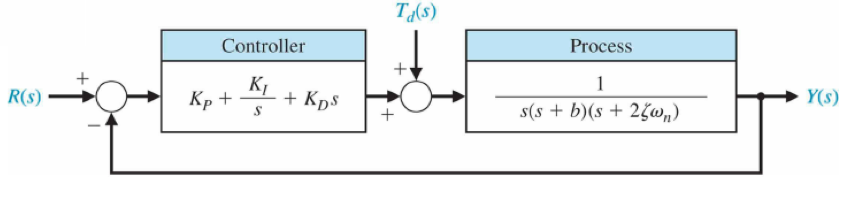
\includegraphics[width=0.6\linewidth]{./figures/e7_9.png}
  \caption{Example system used for the manual tuning example.}
  \label{fig:e7_9}
\end{figure}

\begin{figure} [ht]
  \centering
  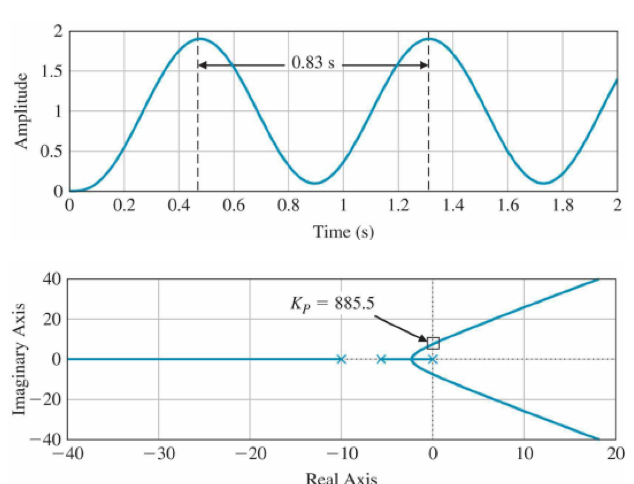
\includegraphics[width=0.5\linewidth]{./figures/e7_91.png}
  \caption{Root locus of P-controller at marginal stability.}
  \label{fig:e7_91}
\end{figure}

\begin{figure} [ht]
  \centering
  \begin{subfigure}[t]{0.3\textwidth}
    \centering
    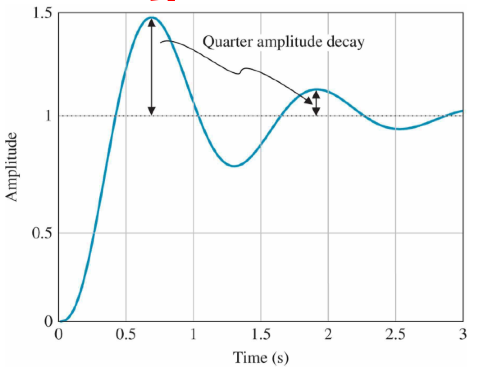
\includegraphics[height=1.4in]{./figures/e7_92.png}
    \caption{Quarter-Amplitude decay case.}
    \label{fig:e7_92}
  \end{subfigure}
  \hfill
  \begin{subfigure}[t]{0.3\textwidth}
    \centering
    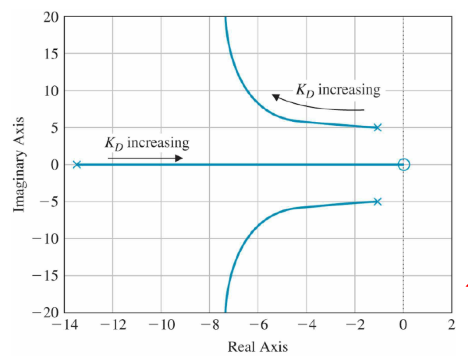
\includegraphics[height=1.4in]{./figures/e7_93.png}
    \caption{Varying $K_D$ in the PD-controller.}
    \label{fig:e7_93}
  \end{subfigure}
  \hfill
  \begin{subfigure}[t]{0.3\textwidth}
    \centering
    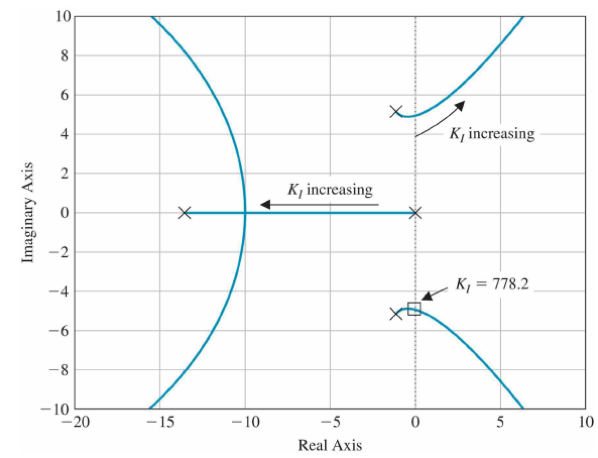
\includegraphics[height=1.4in]{./figures/e7_94.png}
    \caption{Varying $K_I$ in the PI-controller.}
    \label{fig:e7_94}
  \end{subfigure}
\end{figure}

\begin{exa}[Manual Tuning of a PID-controller]
  We consider the system on \Cref{fig:e7_9}.
  Here, the plant has the transfer function
  \begin{equation*}
    G(s) = \frac{1}{s(s+b)(s+2\xi \omega_n}
  \end{equation*}
  with $b = 10, \xi = \num{0,707}, \omega_n = 4$.
  Hence, the process is approximately
  \begin{equation*}
    G(s) = \frac{1}{s(s+10)(s+\num{5,66} )}
  .\end{equation*}
  So the open-loop system has poles at $s = 0, s = -10, s = -\num{5,66}$.
  The pole at the origin means the plant already contains an integrator
  \tcblower
  We start by setting $K_I = K_D = 0$, leaving us with
  \begin{equation*}
    G_c(s) = K_P
  .\end{equation*}
  This gives the closed-loop characteristic equation:
  \begin{equation*}
    1 + K_P \frac{1}{s(s+10)(s+\num{5,66} )} = 0
  \end{equation*}
  or
  \begin{equation*}
    s (s+10)(s+\num{5,66} ) + K_P = 0
  .\end{equation*}
  When $K_P = \num{885,5}$, the closed-loop poles are exactly at $s = \pm \num{7,5} j$, which is exactly on the imaginary axis.
  This is shown on \Cref{fig:e7_91}.

  Here, the response oscillates forever without growing or decaying -- This is also known as marginal stability.
  The oscillation period is approximately $T = 2\pi / \num{7,5}  = \qty{0,84}{\s}$
  Since $K_P = \num{885,5}$ gives sustained oscillation, this is too aggressive.
  We therefore reduce $K_P$ to about 370 to obtain quarter-amplitude decay.
  This is shown on \Cref{fig:e7_92}.

  We now fix $K_P = 370, K_I = 0$ and vary $K_D$, which means the controller is now a PD-controller:
  \begin{equation*}
    G_c(s) = K_P + K_D s
  .\end{equation*}
  The root locus for this is shown on \Cref{fig:e7_93}, where we see that increasing $K_D$ moves the complex poles left, corresponding to faster decay. 

  If we now fix $K_P = 370, K_D = 0$ and instead vary $K_I$ the controller is instead a PI-controller:
  \begin{equation*}
    G_c(s) = K_P + \frac{K_I}{s}
  .\end{equation*}
  On \Cref{fig:e7_94}, we see that increasing $K_I$ moves the complex poles to the right. 
  At $K_I = \num{778,2}$, the system becomes marginally stable with poles at $s = \pm \num{4,86} j$.

  Finally, we choose $K_P = 370, K_I = 100, K_D = 75$ giving the PID-controller
  \begin{equation*}
    G_c(s) = 370 + \frac{100}{s} + 60s = \frac{60s^2 + 370 s + 100}{s}
  .\end{equation*}
  This has the step response depicted on \Cref{fig:e7_95} with overshoot of approximately \num{8,78} \% and settling time of approximately \qty{3,24}{\s}.
\end{exa}

\begin{figure} [ht]
  \centering
  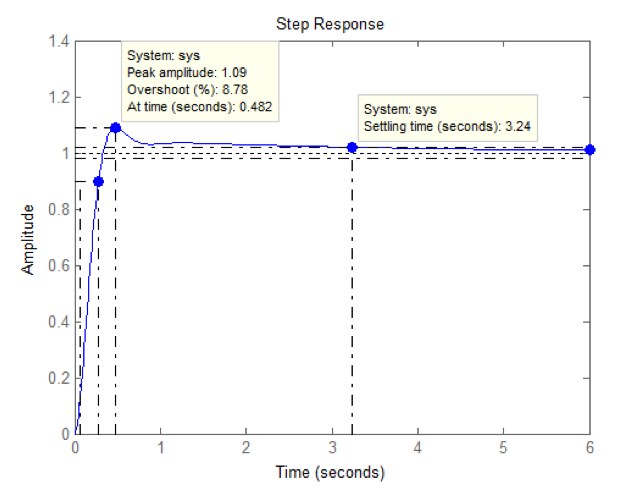
\includegraphics[width=0.6\linewidth]{./figures/e7_95.png}
  \caption{Manually tuned PID-controller.}
  \label{fig:e7_95}
\end{figure}

\subsubsection{Closed-loop Ziegler-Nichols PID Tuning}
Ziegler-Nichols tuning is a rule-based way to get initial PID gains without needing a perfect mathematical model of the process.
We generally distinguish between closed-loop and open-loop Ziegler Nichols tuning. Closed-loop Ziegler-Nichols tuning uses the closed-loop system and finds the ultimate gain and ultimate period, whereas open-loop Ziegler-Nichols tuning uses the open-loop step response, also called the reaction curve.
Here, we focus on the closed-loop Ziegler-Nichols method.

The method starts like manual tuning with $K_I = K_D = 0$, so the controller is initially only proportional:
\begin{equation*}
  G_c(s) = K_P
.\end{equation*}
Then $K_P$ is increased, until the closed-loop system is on the boundary of instability, i.e. marginal stability.
At this point we measure two things, $K_U$ which is the ultimate gain (the value of $K_P$ that gives sustained oscillations), and the ultimate period $T_U$ (the period of the sustained oscillations).

The closed-loop Ziegler-Nichols rules are shown on \Cref{tab:ZN}.
\begin{table}[ht]
  \caption{Closed-loop Ziegler-Nichols rules}
  \label{tab:ZN}
  \centering
  \begin{tabular}{|c|c|c|l|}
    \hline
    \textbf{Controller} & \textbf{$K_P$}  & \textbf{$K_I$}              & \textbf{$K_D$}               \\ \hline
    P                   & $\num{0,5}K_U$  & --                          & --                           \\ \hline
    PI                  & $\num{0,45}K_U$ & $\frac{\num{0,54}K_U}{T_U}$ & --                           \\ \hline
    PID                 & $\num{0,6}K_U$  & $\frac{\num{1,2}K_U}{T_U}$  & $ \frac{\num{0,6}K_UT_U}{s}$ \\ \hline
  \end{tabular}
\end{table}

\begin{exa}[Ziegler-Nichols Tuning of a PID-controller]
  We use the same process as before:
  \begin{equation*}
    G(s) = \frac{1}{s(s+b)(s+2\xi \omega_n)} = \frac{1}{s(s+10)(s+\num{5,66} )}
  .\end{equation*}
  \tcblower
  With $K_I = K_D = 0$, the closed-loop characteristic equation is
  \begin{equation*}
    1 + K_P \frac{1}{s(s+10)(s+\num{5,66} )} = 0
  .\end{equation*}
  When $K_P = \num{885,5}$ the system is at marginal stability and the closed-loop poles are at $s = \pm\num{7,5}j $ as shown on \Cref{fig:e7_91}.
  Therefore $K_U = \num{885,5}$ and the period of oscillation here is $T_U = \qty{0,84}{\s}$. 

  Using the PID-row of \Cref{tab:ZN}, we see that:
  \begin{gather*}
    K_P = \num{0,6} K_U = \num{531,3} \\
    K_I = \frac{\num{1,2} K_U}{T_U} = \num{1280,2} \\
    K_D = \frac{\num{0,6} K_U T_U}{8} = \num{55,1} 
  .\end{gather*}
  So using Ziegler-Nichols tuning the PID controller becomes
  \begin{equation*}
    G_c(s) = \num{531,3}  + \frac{\num{1280,2}}{s} + \num{55,1} s = \frac{\num{55,1} s^2 + \num{531,2}s + \num{1280,2} }{s}
  .\end{equation*}
  This gives the step response on \Cref{fig:e7_10}, where it is compared with the result from the manual tuning on \Cref{fig:e7_952}.
\end{exa}

\begin{figure} [ht]
  \centering
  \begin{subfigure}[t]{0.48\textwidth}
    \centering
    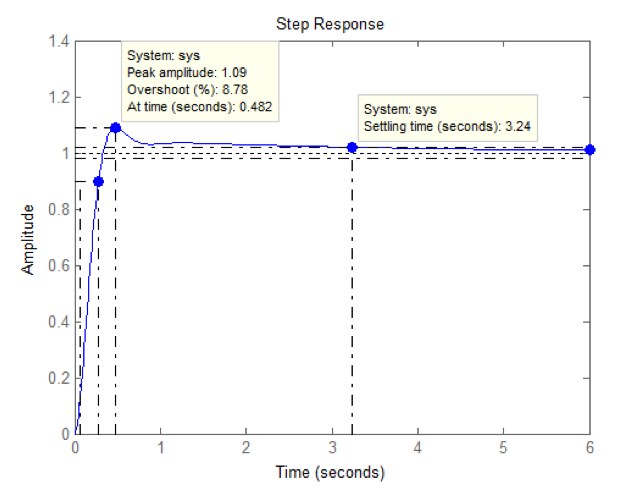
\includegraphics[height=2in]{./figures/e7_95.png}
    \caption{Step response from Manual tuning.}
    \label{fig:e7_952}
  \end{subfigure}
  \hfill
  \begin{subfigure}[t]{0.48\textwidth}
    \centering
    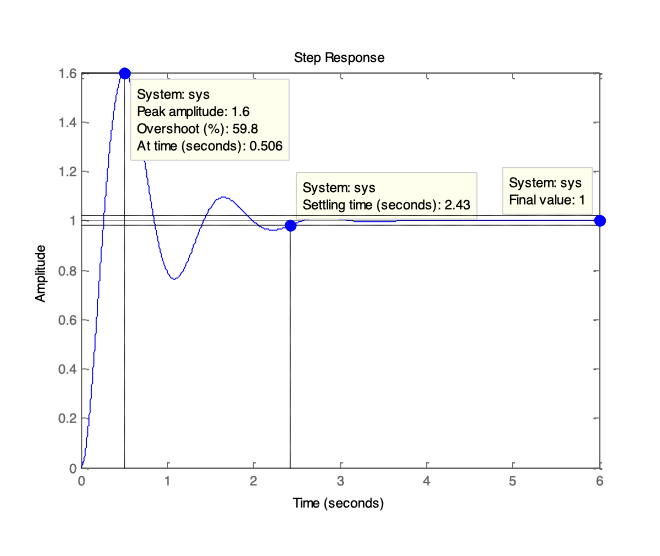
\includegraphics[height=2.2in]{./figures/e7_10.png}
    \caption{Step response from Ziegler-Nichols tuning.}
    \label{fig:e7_10}
  \end{subfigure}
  \caption{Comparison of step responses between manually tuned and Ziegler-Nichols tuned PID controller.}
  \label{fig:tuncomp}
\end{figure}

On \Cref{fig:tuncomp} the step responses from the manually tuned on the Ziegler-Nichols tuned PID controllers are shown. 
Here, we see that the manual tuning has much less overshoot but a bit longer settling time than the Ziegler-Nichols tuned PID controller.


\begin{exa}[Automobile Velocity Control]
  We define $y(t)$ to be the relative velocity between two vehicles, and our plant is modeled as
  \begin{equation*}
    G(S) = \frac{1}{(s+2)(s+8)}
  \end{equation*}
  so the open-loop system has two stable poles at $s = -2$ and $s = -8$. 
  The controller must satisfy four requirements:
  \begin{enumerate}
    \item Zero steady-state error to a step input
    \item Steady-state error to a ramp input less than 25\%
    \item Percent overshoot less than 5\%
    \item Settling time less than \qty{1,5}{\s} 
  \end{enumerate}
  \tcblower
  We start by considering the first design spec: zero steady state error to a step.
  The plant is
  \begin{equation*}
    G(s) = \frac{1}{(s+2)(s+8)}
  \end{equation*}
  so we have no poles at the origins and hence a type 0 system.
  For zero steady state error to a step input, the open-loop system must be at least type 1, meaning it needs one integrator $1 / s$. 
  Therefore, the controller must be a type 1 controller to provide this integrator.
  For this, we choose a PI controller:
  \begin{equation*}
    G_c(s) = K_P + \frac{K_I}{s} = \frac{K_P s + K_I}{s}
  .\end{equation*}
  
  For the second spec; the ramp error condition, we remember that steady-state error to a ramp input is related to the velocity error constant:
  \begin{equation*}
    K_v = \lim_{s \to 0}s G_c(s) G(s)
  .\end{equation*}
  We require that the error is less than 25\% so $K_v > 1 / \num{0,25}  = 4$.
  Now, using the PI controller and the plant:
  \begin{equation*}
    G_C(s) = \frac{K_P s + K_I}{s} \qquad G(s) = \frac{1}{(s+2)(s+8)}
  .\end{equation*}
  Then:
  \begin{equation*}
    K_v = \lim_{s \to 0} s \frac{K_P s + K_I}{s} \frac{1}{(s+2)(s+8)} = \lim_{s \to 0} \frac{K_P s + K_I}{(s+2)(s+8)}
  .\end{equation*}
  At $s = 0$:
  \begin{equation*}
    K_v = \frac{K_I}{2\cdot 8} = \frac{K_I}{16} \implies \frac{K_I}{16} > 4 \implies K_I > 64
  .\end{equation*}
  
  For the overshoot condition, we look at the damping ratio $\xi$.
  The requirement here is $M_P < 5\%$, which corresponds approximately to $\xi \geq \num{0,69} $.
  So the closed-loop dominant poles should lie in the region of the $s$-plane corresponding to a damping ratio of at least \num{0,69}.

  To look at the settling time condition we remember that 2\% settling time is approximately:
  \begin{equation*}
    T_s \approx \frac{4}{\xi \omega_n}
  .\end{equation*}
  We require $T_s \leq \num{1,5}$, so
  \begin{align*}
    \frac{4}{\xi \omega_n} &\leq \num{1,5} \\
    \xi \omega_n &\geq \num{2,67} 
  .\end{align*}
  The real part of a complex pole pair is $\Re(s) = - \xi \omega_n$, so the dominant poles should be to the left of $s \approx - \num{2,6}$. 

  The open-loop transfer function is:
  \begin{equation*}
    G_c(s) G(s) = \frac{K_P s + K_I}{s(s+2)(s+8)}
  .\end{equation*}
  The closed-loop transfer function is:
  \begin{equation*}
    T(S) = \frac{G_c(s) G(s)}{1 + G_c(s) G(s)}
  .\end{equation*}
  Substituting gives:
  \begin{equation*}
    T(s) = \frac{K_P s + K_I}{s(s+2)(s+8) + K_P s + K_I} = \frac{K_P s + K_I}{s^3 + 10s^2 + (16 + K_P)s + K_I}
  .\end{equation*}
  
  We now apply the Routh-Hurwitz criterion to the characteristic equation:
  \begin{equation*}
    s^3 + 10s^2 + (16 + K_P)s + K_I = 0
  .\end{equation*}
  The Routh table gives the stability conditions:
  \begin{align*}
    K_I &> 0 \\
    K_P &>  \frac{K_I}{10} - 16
  .\end{align*}
  So to be stable $K_I$ must be positive and $K_P$ must be large enough relative to $K_I$.
  From spec 2 we have $K_I > 64$, so
  \begin{align*}
    K_I &> 64 \\
    K_P &>  \frac{K_I}{10} - 16
  .\end{align*}

  The open-loop transfer function can be written as
  \begin{equation*}
    G_c(s) G(s) = K_P \frac{s + \frac{K_I}{K_P}}{s(s+2)(s+8)}
  .\end{equation*}
  Which has poles at $s = 0$, $s = -2$, $s=-8$ and a zero at $s = - K_I / K_P$.
  The asymptote angles are $\phi_A = +\ang{90}, -\ang{90}$. 
  The asymptote centroid is
  \begin{equation*}
    \sigma_A = \frac{\sum \text{poles} - \sum \text{zeros}}{n_p - n_z} = \frac{0-2-8- \left( - \frac{K_I}{K_P} \right)}{2} = -5 + \frac{K_I}{2K_P}
  .\end{equation*}
  
  We now use spec 4 to choose a location for our zero.
  To meet the settling time requirement, the dominant poles should be left of $s = - \num{2,6}$.
  We use the asymptote centroid as a root-locus design guide and require:
  \begin{align*}
    \sigma_A &< -\num{2,6} \\
    -5 + \frac{K_I}{2K_P} &< \num{2,4} \\
    \frac{K_I}{K_P} &< \num{4,8} 
  .\end{align*}
  We choose $K_I / K_P = \num{2,5}$, which means the PI zero is located at $s = - \num{2,5}$ so the root locus becomes:
  \begin{equation*}
    1 + K_P \frac{s + \num{2,5} }{s(s+2)(s+8)} = 8
  .\end{equation*}
  With the zero fixed at $-\num{2,5}$, the root locus can be plotted as shown on \Cref{fig:e7_16}, where the desired region is shaded.
  We conclude that $K_P < 30$ is required.

  Therefore our final gain conditions are
  \begin{align*}
    K_I &> 64 \\
    K_P &< 30 \\
    \frac{K_I}{K_P} &= \num{2,5}
  .\end{align*}
  Therefore we need $\num{2,5} K_P > 64 \implies K_P > \num{25,6}$. 
  Together with $K_P < 30$, a reasonable choice is $K_P = 26$, and then $K_I = \num{2,5} \cdot 26 = 65$, so our final PID controller is
  \begin{equation*}
    G_c(s) = 26 + \frac{65}{s} = \frac{26s + 65}{s}
  .\end{equation*}
  The final closed-loop transfer function is then:
  \begin{equation*}
    T(s) = \frac{26s + 65}{s^3 + 10s^2 + 42 s + 65}
  .\end{equation*}
  The final step response is shown on \Cref{fig:e7_162}.
\end{exa}

\begin{figure} [ht]
  \centering
  \begin{subfigure}[t]{0.48\textwidth}
    \centering
    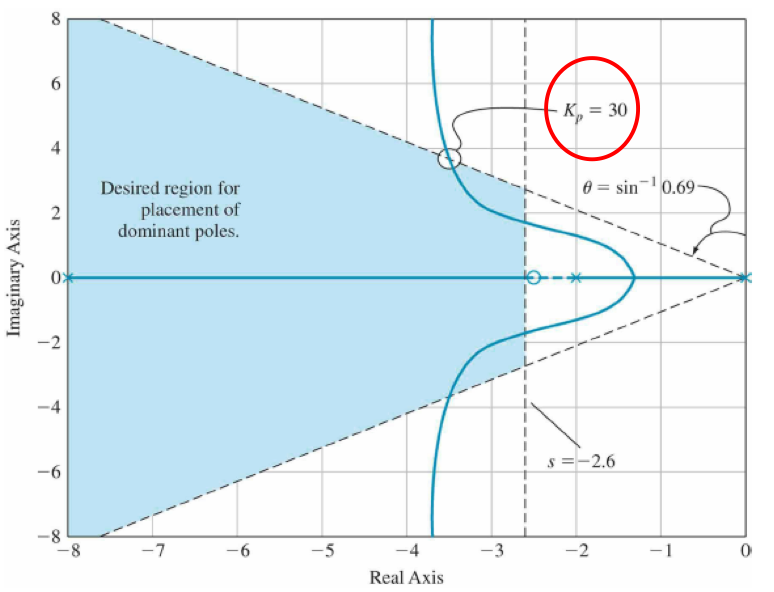
\includegraphics[height=2in]{./figures/e7_16.png}
    \caption{Root Locus with fixed zero at $-\num{2,5}$.}
    \label{fig:e7_16}
  \end{subfigure}
  \hfill
  \begin{subfigure}[t]{0.48\textwidth}
    \centering
    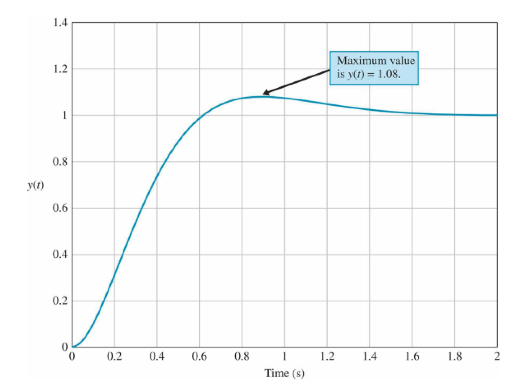
\includegraphics[height=2in]{./figures/e7_162.png}
    \caption{Final step response.}
    \label{fig:e7_162}
  \end{subfigure}
\end{figure}
